% Template for PLoS
% Version 3.3 June 2016
%
% % % % % % % % % % % % % % % % % % % % % %
%
% -- IMPORTANT NOTE
%
% This template contains comments intended 
% to minimize problems and delays during our production 
% process. Please follow the template instructions
% whenever possible.
%
% % % % % % % % % % % % % % % % % % % % % % % 
%
% Once your paper is accepted for publication, 
% PLEASE REMOVE ALL TRACKED CHANGES in this file 
% and leave only the final text of your manuscript. 
% PLOS recommends the use of latexdiff to track changes during review, as this will help to maintain a clean tex file.
% Visit https://www.ctan.org/pkg/latexdiff?lang=en for info or contact us at latex@plos.org.
%
%
% There are no restrictions on package use within the LaTeX files except that 
% no packages listed in the template may be deleted.
%
% Please do not include colors or graphics in the text.
%
% The manuscript LaTeX source should be contained within a single file (do not use \input, \externaldocument, or similar commands).
%
% % % % % % % % % % % % % % % % % % % % % % %
%
% -- FIGURES AND TABLES
%
% Please include tables/figure captions directly after the paragraph where they are first cited in the text.
%
% DO NOT INCLUDE GRAPHICS IN YOUR MANUSCRIPT
% - Figures should be uploaded separately from your manuscript file. 
% - Figures generated using LaTeX should be extracted and removed from the PDF before submission. 
% - Figures containing multiple panels/subfigures must be combined into one image file before submission.
% For figure citations, please use "Fig" instead of "Figure".
% See http://journals.plos.org/plosone/s/figures for PLOS figure guidelines.
%
% Tables should be cell-based and may not contain:
% - spacing/line breaks within cells to alter layout or alignment
% - do not nest tabular environments (no tabular environments within tabular environments)
% - no graphics or colored text (cell background color/shading OK)
% See http://journals.plos.org/plosone/s/tables for table guidelines.
%
% For tables that exceed the width of the text column, use the adjustwidth environment as illustrated in the example table in text below.
%
% % % % % % % % % % % % % % % % % % % % % % % %
%
% -- EQUATIONS, MATH SYMBOLS, SUBSCRIPTS, AND SUPERSCRIPTS
%
% IMPORTANT
% Below are a few tips to help format your equations and other special characters according to our specifications. For more tips to help reduce the possibility of formatting errors during conversion, please see our LaTeX guidelines at http://journals.plos.org/plosone/s/latex
%
% For inline equations, please be sure to include all portions of an equation in the math environment.  For example, x$^2$ is incorrect; this should be formatted as $x^2$ (or $\mathrm{x}^2$ if the romanized font is desired).
%
% Do not include text that is not math in the math environment. For example, CO2 should be written as CO\textsubscript{2} instead of CO$_2$.
%
% Please add line breaks to long display equations when possible in order to fit size of the column. 
%
% For inline equations, please do not include punctuation (commas, etc) within the math environment unless this is part of the equation.
%
% When adding superscript or subscripts outside of brackets/braces, please group using {}.  For example, change "[U(D,E,\gamma)]^2" to "{[U(D,E,\gamma)]}^2". 
%
% Do not use \cal for caligraphic font.  Instead, use \mathcal{}
%
% % % % % % % % % % % % % % % % % % % % % % % % 
%
% Please contact latex@plos.org with any questions.
%
% % % % % % % % % % % % % % % % % % % % % % % %

\documentclass[10pt,letterpaper]{article}
\usepackage[top=0.85in,left=2.75in,footskip=0.75in]{geometry}

% amsmath and amssymb packages, useful for mathematical formulas and symbols
\usepackage{amsmath,amssymb}

% Use adjustwidth environment to exceed column width (see example table in text)
\usepackage{changepage}

% Use Unicode characters when possible
\usepackage[utf8x]{inputenc}

% textcomp package and marvosym package for additional characters
\usepackage{textcomp,marvosym}

% cite package, to clean up citations in the main text. Do not remove.
\usepackage{cite}

% Use nameref to cite supporting information files (see Supporting Information section for more info)
\usepackage{nameref,hyperref}

% line numbers
\usepackage[right]{lineno}

% ligatures disabled
\usepackage{microtype}
\DisableLigatures[f]{encoding = *, family = * }

% color can be used to apply background shading to table cells only
\usepackage[table]{xcolor}

% array package and thick rules for tables
\usepackage{array}

% create "+" rule type for thick vertical lines
\newcolumntype{+}{!{\vrule width 2pt}}

% create \thickcline for thick horizontal lines of variable length
\newlength\savedwidth
\newcommand\thickcline[1]{%
  \noalign{\global\savedwidth\arrayrulewidth\global\arrayrulewidth 2pt}%
  \cline{#1}%
  \noalign{\vskip\arrayrulewidth}%
  \noalign{\global\arrayrulewidth\savedwidth}%
}

% \thickhline command for thick horizontal lines that span the table
\newcommand\thickhline{\noalign{\global\savedwidth\arrayrulewidth\global\arrayrulewidth 2pt}%
\hline
\noalign{\global\arrayrulewidth\savedwidth}}


% Remove comment for double spacing
%\usepackage{setspace} 
%\doublespacing

% Text layout
\raggedright
\setlength{\parindent}{0.5cm}
\textwidth 5.25in 
\textheight 8.75in

% Bold the 'Figure #' in the caption and separate it from the title/caption with a period
% Captions will be left justified
\usepackage[aboveskip=1pt,labelfont=bf,labelsep=period,justification=raggedright,singlelinecheck=off]{caption}
\renewcommand{\figurename}{Fig}

% Use the PLoS provided BiBTeX style
\bibliographystyle{plos2015}

% Remove brackets from numbering in List of References
\makeatletter
\renewcommand{\@biblabel}[1]{\quad#1.}
\makeatother

% Leave date blank
\date{}

% Header and Footer with logo
\usepackage{lastpage,fancyhdr,graphicx}
\usepackage{epstopdf}
\pagestyle{myheadings}
\pagestyle{fancy}
\fancyhf{}
\setlength{\headheight}{27.023pt}
\lhead{
\includegraphics[width=2.0in]{PLOS-submission.eps}}
\rfoot{\thepage/\pageref{LastPage}}
\renewcommand{\footrule}{\hrule height 2pt \vspace{2mm}}
\fancyheadoffset[L]{2.25in}
\fancyfootoffset[L]{2.25in}
\lfoot{\sf PLOS}

%% Include all macros below

\newcommand{\lorem}{{\bf LOREM}}
\newcommand{\ipsum}{{\bf IPSUM}}

%% END MACROS SECTION


\begin{document}
\vspace*{0.2in}

% Title must be 250 characters or less.
\begin{flushleft}
{\Large
\textbf\newline{Measuring Aspects of the Web Browser Ecosystem} % Please use "title case" (capitalize all terms in the title except conjunctions, prepositions, and articles).
}
\newline
% Insert author names, affiliations and corresponding author email (do not include titles, positions, or degrees).
\\
Sela Ferdman\textsuperscript{1},
Einat Minkov\textsuperscript{2},
Ron Bekkerman\textsuperscript{3},
David Gefen\textsuperscript{4}
%Name5 Surname\textsuperscript{2\ddag},
%Name6 Surname\textsuperscript{2\ddag},
%Name7 Surname\textsuperscript{1,2,3*},
%with the Lorem Ipsum Consortium\textsuperscript
%{\textpilcrow}
\\
\bigskip
\textbf{1} Department of Computer Science, University of Haifa, Israel
\\
\textbf{2} Department of Information Systems, University of Haifa, Israel
\\
\textbf{3} Department of Information and Knowledge Management, University of Haifa, Israel
\\
\textbf{4} LeBow College of Business, Drexel University, Philadelphia PA, USA
\\
\bigskip

% Insert additional author notes using the symbols described below. Insert symbol callouts after author names as necessary.
% 
% Remove or comment out the author notes below if they aren't used.
%
% Primary Equal Contribution Note
%\Yinyang These authors contributed equally to this work.

% Additional Equal Contribution Note
% Also use this double-dagger symbol for special authorship notes, such as senior authorship.
%\ddag These authors also contributed equally to this work.

% Current address notes
%\textcurrency Current Address: Dept/Program/Center, Institution Name, City, State, Country % change symbol to "\textcurrency a" if more than one current address note
% \textcurrency b Insert second current address 
% \textcurrency c Insert third current address

% Deceased author note
%\dag Deceased

% Group/Consortium Author Note
%\textpilcrow Membership list can be found in the Acknowledgments section.

% Use the asterisk to denote corresponding authorship and provide email address in note below.
%* correspondingauthor@institute.edu

\end{flushleft}
% Please keep the abstract below 300 words
\section*{Abstract}
Contrary to the assumption that web browsers are designed to support the user, an examination of a 900,000 distinct PCs shows that web browsers comprise a complex ecosystem with millions of \textit{addons} competing and collaborating with each. Addons ``sneak in'' through third party installations and others are ``kicked out'' by their competitors without user involvement. This study examines this ecosystem by constructed a large-scale graph with nodes corresponding to users, addons, and words (terms) extracted from addons' attributes. Running a Personalized PageRank (PPR) random walk to traverse this graph shows that the graph demonstrates \textit{ecological resilience}. Adapting the PPR model to analyzing the browser ecosystem at the level of addon manufacturer, the study shows that some addon companies are in \textit{symbiosis} and others \textit{clash} with each other as shown by analyzing the behavior of 18 prominent addon manufacturers. Results may herald insight on how other evolving internet ecosystems may behave, and suggest a methodology for measuring this behavior. 


% Please keep the Author Summary between 150 and 200 words
% Use first person. PLOS ONE authors please skip this step. 
% Author Summary not valid for PLOS ONE submissions.   
%\section*{Author Summary}

\linenumbers

% Use "Eq" instead of "Equation" for equation citations.
\section*{Introduction}

Web browser behavior is beginning to resemble AI in that browser addons are making their own decisions independently and often unbeknown to the user. User-independent machine decision-making impose questions that have traditionally been discussed in science fiction but are now being brought to the spotlight of public attention. In their seminal paper, Russell et. al.~\cite{russell2016research} posed such questions, mostly related to the legal, ethical, and structural regulation of decisions that can be made by intelligent systems. That paper led to formulating a widely recognized Open Letter on research priorities for robust and beneficial AI, signed so far by over 8000 scientists and technologists (including Stephen Hawking, Bill Gates, and Elon Musk). The goal of that open letter is clear: ``our AI systems must do what we want them to do''. Amodei et al.~\cite{amodei2016concrete} went further into some practical aspects of achieving this goal, proposing concrete methods for minimizing damage that an intelligent system may cause to its environment. 

What is less clear, however, is how this goal can be achieved. While Amodei et al.'s paper paves a way to building harmless AI, it makes it apparent that not all possible problems can be identified and immediately solved. The world in which both humans and machines are first-class citizens seems to be more complex than could have been imagined. The field of Human-Computer Interaction~\cite{dix2009human} has mostly been concerned with how one human communicates with one machine, or how humans communicate with each other with the help of machines. Multi-Agent Systems research (e.g.,~\cite{olfati2007consensus}), likewise, deals with cooperation between machines, while overly ignoring the environments in which machines do not want to cooperate with each other, are not designed to cooperate with each other, or are simply unaware of each other. Nevertheless, those are the most common environments.

The objective of this paper is to show the applicability of running a Personalized PageRank (PPR) random graph walk in the context of web browser behavior to \textit{quantify} such independent machine behavior. That could be a first step toward monitoring and regulating independent machine behavior. This quantification sheds new light on the coexistence of machines with other machines. The proposed quantification is shown in the context of web browser addons. This allows for its demonstration in a known and relatively simple context. Web browsers have become a major component of the routine human-computer interaction, with some operating systems based entirely on browsers (e.g., ChromeOS by \textit{Google}).\footnote{ http://www.chromium.org/chromium-os} Browser \textit{extensions}, also known as \textit{addons}, are computer programs that (as the name suggests) extend, improve, and personalize browser capabilities. Addons compete with each other over resources (battery, memory, disk space, computing power) and user attention. More than 750 million (non-unique) addons were downloaded and installed by \textit{Google} Chrome browser users as of June 2012.\footnote{ http://www.medianama.com/2012/06/223-the-lowdown-google-io-2012-day-2-310m-chrome-users-425m-gmail-more/} Addons, regardless of how intelligent they are, may be aware of each other and may be designed to compete with each other independently of the user.\footnote{Extensions serve a wide variety of purposes. Some examples of those include an extension that allows visually impaired users to access the content of bar charts on the Web~\cite{elzer2007browser}, an addon that addresses users' security concerns by seamlessly producing a unique password for each website the user accesses~\cite{ross2005stronger}.} 

An example of independent machine behavior in the context of addons is an antivirus tool that is being installed on a laptop: what should it do about another antivirus tool that was preinstalled on that laptop? Such questions are becoming more pertinent because while browser extensions can be installed proactively, they are often `silently' installed on one's machine by a third party, typically, as the user downloads some other program or installs a 'software bundle'. This is also a question of much economic impact. Internet software companies are very interested in installing their addons, and particularly toolbars, on users' machines. Toolbars are GUI widgets that typically reside in the upper part of the browser's window, extending the browser's functionality. Toolbars can collect information about the browsing history of the user (e.g., Yahoo!~Toolbar\footnote{ https://www.google.com/patents/US8375131}) and can redirect user search activity to a specific search portal (e.g. MyWebSearch.com). Crucially, the company that owns the search portal, and typically also the toolbar, receives payments from ad providers per user click on the ads it displays (primary ad providers are \textit{Google} and \textit{Yahoo!}). This revenue generation model is used extensively by software companies that distribute freeware products~\cite{leontiadis2012don}. For example, 45\% of AVG Technologies sales in 2012 were generated by its browser toolbar.\footnote{ http://seekingalpha.com/article/1147451} It was estimated that \textit{Google}, the biggest Web advertising firm, might have lost \$1.3 billion in revenue in 2013 because of changes to its policy with respect to toolbars and a resulting shift of some addon distributors to \textit{Google}'s competitors.\footnote{ http://finance.yahoo.com/news/google-may-miss-2013-revenue-113926474.html}$^{,}$\footnote{ https://support.google.com/adwordspolicy/answer/50423?hl=en}

One way to conceptualize independent machine behavior in the context of addons is to look at it through the lenses of \textit{Digital Ecology}~\cite{kleineberg2015digital} which conveniently has been expanded into \textit{Cyber-Physical-Socio Ecology}~\cite{shi2011cyber}. To the best of our knowledge, no empirical study to date has tried to establish a direct connection between ecology and this new bio-digital environment. In this paper we show that some aspects of the digital environment seem to obey the rules of traditional ecology. With the Web browser environment being a prominent example of machine-to-machine ecosystems, drawing parallels with the better understood biologically ecosystems might present a viable way of thinking about such systems. To the extent that the Internet of Things might be developing a similar ecology, Web browser ecology may be a herald of things to come.  

\section*{Research Questions and their Addon Ecosystem Context}

The Web browser ecosystem is a complex evolving one. Addons are installed and uninstalled on user machines. New addons introduced by software companies become prevalent or fade over time. New addon companies enter, and older players gain or lose power. Companies establish partnerships or compete with each other (and sometimes both). To mention but a few of its dynamic characteristics. All this happens on a daily basis and is mostly hidden from the user who may not even be aware of the vibrant ``life'' on his/her Web browser. These developments occur solely within the digital media---addons being software executables---with each addon having a lifecycle of events and a spectrum of interactions with its environment. 

Addons are in a symbiotic relationship when at least one of them benefits from the other. For example, an addon may get installed on a user's machine during (or following) the installation of another addon. This can be considered a direct benefit to the addon, as it would not have reached the machine if the other addon was not installed on it. Often, addons of the same company are installed in a bundle. In some cases, addons companies may even have a distribution agreement such that one company provides the means for installing the other company's addons. Clashes occur when an addon ``kicks out'' other addons. There are a variety of reasons for a clash. A clash may happen, for example, when one company's addon removes another company's addon because the two companies' products directly compete with each other. Of course, also the user (i.e. the computer owner) may be playing an important role in the addon ecosystem: some users ``hunt down'' and remove addons that occasionally appear in the computer's browser; other users are more tolerant---they let addons live in the browser for a long time and do not mind more addons to be installed over time. 

All these processes occur in the Web browser \textit{habitat}. This habitat is observably \textit{ecologically stable} (browsers do not crash frequently) and shows \textit{resilience}: if not disturbed, the habitat will remain approximately the same, and if disturbed from outside then it will ``remember'' its stable state and try to recover. 

Addressing the research objective of quantifying independent machine behavior in the context of addon ecosystems, the first research question aims to establish that habitat resilience can be measured, and then, building on that verification, the next research questions address the symbiosis and clash characteristics of that habitat. 


\noindent \textbf{RQ1: Can Web browser habitat resilience be verified?}

\noindent \textbf{RQ2: Can the degree of addon symbiosis and clash be measured?}

The research questions are addressed by analyzing records of user-addon associations collected from anonymous users all over the world. The original data consisted of addon textual descriptions and their installation paths. That data was cast into a relational graph in which typed nodes correspond to distinct \textit{user}, \textit{addon}, and \textit{term} objects. In this representation a habitat observed on an individual user's machine forms a star-shaped graph in which a node corresponding to the \textit{user} is linked to nodes corresponding to the \textit{addons} that reside on that user's machine. Those \textit{addon} nodes may be further linked to lexical\textit{ terms}, derived from their textual descriptions. Multiple habitats can be represented in a joint graph. For example, each \textit{addon} can be directly connected to all the \textit{users} that have it installed. The graph representation is compact, supporting efficient processing of large-scale data. Importantly, graph-theoretic methods can be employed to assess structural inter-node relatedness.

The ability to verify habitat resilience (RQ1) is measured by showing that if a random addon is removed from the habitat then, given the identity of the remaining addons in that habitat and inter-habitat relationships as registered on the relational graph, the missing addon can be identified. The statistical significance of being able to do so is shown by verifying that a Personalized PageRank (PPR) random walk is significantly better than a `one-fits-all' methods such as the \textit{popular choice} method. Given that habitat resilience can be verified, the subsequent RQ2 research question shows that two defining characteristics of a habitat, symbiosis and clash, can also be measured by assessing the relationships among addon companies. A graph-based measure of \textit{conditional importance} is employed for this purpose.

The results show that habitat resilience and the degree of addon symbiosis and clash can be measured. Being able to measure these may open the door to further research to monitor independent machine behavior. The results also suggest that PPR may be a candidate algorithm for doing so, and show its ability to detect business alliances and rivalries in digital media. 


\section*{Related Research}

Gaining insight from biology to computer science is a topic of ongoing research~\cite{rasmus2015computational}. Examples include the popular analogy of malicious software to viruses~\cite{cohen1987computer}, the study of epidemic propagation in networks~\cite{christosKAIS14}, the comparison of information dissemination on social networks to an evolutionary process (Adamic et. al. 2016), and more. This study follows in the footsteps of previous research that outlined an analogy between biological ecosystems and the collective behavior of players, or processes, in the software industry. While that literature, discussed next, is theoretical and anecdotal, this study reports empirical results using real-world data that shows characteristics of software ecosystems similar to those of biological ecosystems. The next sections will define ecosystems in the context of previous research, and then survey research related to the methodology used in this study.

\subsection*{Business and Software Ecosystems}

It has long been suggested that companies should not be viewed as individual entities, but rather as part of a \textit{business ecosystem} \cite{moore93,iansiti04}. Applying this paradigm, companies might be thought of as corresponding to species in a biological ecosystem. Like its biological counterpart, a business ecosystem is assumed to gradually develop from a collection of elements to a structured community, and, likewise, each member of a business ecosystem ultimately shares the fate of the network as a whole, regardless of its relative strength. 

To put this study into perspective, we overview recent research focused on \textit{software ecosystems} \cite{messerschmitt2005software,dhungana2010software, manikas13,jansen13}, studying the complex relationships among companies in the software industry. Manikas and Hansen~\cite{manikas13} defined a software ecosystem as the interaction of a set of actors on top of a common technological platform that results in a number of software solutions or services. As an example, they considered the iOS ecosystem in which \textit{Apple} provides a platform for selling applications in return for a yearly fee and 30\% of revenues of application sale. According to Manikas and Hansen, software ecosystems are characterized with a wide spectrum of symbiotic relationships: two actors might have mutual benefits, be in direct competition (antagonism), be unaffected (neutralism), or be in a position where one company is unaffected while the other is benefiting (amensalism) or harmed (parasitism) by their relationship. Manikas and Hansen noted that little research had been done in the context of real-world ecosystems. Other researchers used the term `software ecosystems' to describe more technical aspects concerning the development of software systems that involves multiple players and must adapt to new environment or requirements \cite{lunguPhd09,blincoeMSR15}. 

To the best of our knowledge, the current work is the first that studies interactions between players in the Web browsers addons domain. This Web browser ecosystem differs from organization-centric software ecosystems previously studied in the literature (e.g., \cite{christensen2014analysis}) where an organization develops a software ecosystem around its offering, such as in the case of \textit{Salesforce} that created a marketplace of third-party extensions to its products~\cite{jansen2013defining}. In the Web browser ecosystem there is no organization that can regulate addon behavior. Moreover, browser addons can interact directly with each other, even removing each other from the user's machine, which is not allowed in a the regulated ecosystem of an organization. Jansen and Cusumano~\cite{jansen2013defining} found that a significant difference between the software and ecological ecosystems is that software species can `consciously' decide to exit the ecosystem as opposed to species in a biological ecosystem. That distinction, however, may not readily apply to the browser addon ecosystem because addons do not leave the system at their own will---once installed, only external factors limit their survival. 

The resilience of a biological ecosystem is defined as the amount of disturbance that it can withstand without changing its self-organized processes and structures~\cite{holling1973resilience}, or as the time required for the ecosystem to return to its stable state after a perturbation~\cite{tilman1996biodiversity}. Dhungana et. al.~\cite{dhungana2010software} define a sustainable software ecosystem as one that can survive a significant habitat changes coming from competitors. Along the same lines, this study defines ecological resilience as the ability of a Web browser ecosystem that is artificially disturbed by extracting an existing addon to ``remember'' its original state to the extent that the missing addon can be predicted. Such \textit{ecological memory} is a main component of ecological resilience, playing a major role in reorganization of ecosystems~\cite{gunderson2000ecological}. Ecological memory includes the biological legacies within habitat and the genetic composition of populations. As described by Schaefer~\cite{schaefer2009alien}, ecological memory is encapsulated in soil properties, spores, seeds, stem fragments, species, populations and other remnants that influence the composition of the replacement ecosystem and may also support ecological restoration. In particular, an internal component of ecological memory consists of remnants of species in the immediate area and an external component consists of the surrounding areas. 

\subsection*{Graph-based data representation}

The definitions above imply that an ecosystem can be presented as a set of objects that interact in various ways among themselves, and possibly with other environmental objects. Such relational schema is naturally represented using a heterogeneous typed graph in which nodes denote entities and edges denote inter-entity relationships~\cite{minkov2010improving,sunWSDM12}. A plethora of well-studied and efficient methods exists that can identify global phenomena in such a graph and evaluate the relatedness between remote entity pairs~\cite{kleinberg07,sun12}. Nonetheless, only few studies analyzed ecosystems using quantifiable measures. One such study was conducted by Blincoe et. al.~\cite{blincoeMSR15} who aimed at identifying ecosystems among software projects developed in the \textit{GitHub} platform.\footnote{ https://github.com/} Blincoe et. al. constructed a graph in which vertices denoted software projects on \textit{GitHub} and edges represented technical cross-project references. Multi-project ecosystems in their graph were then identified using a community detection method and displayed visually. This study takes graphing ecosystems a step further. The current study uses quantifiable graph measures to establish that addons form an ecosystem that is resilient and then to detect collaboration and adversary relations between the members of the ecosystem.

To establish that addons form an ecosystem that is resilient, resilience is formalized as a \textit{link prediction} problem. The general task of link prediction aims at estimating whether a link should exist between two disconnected nodes in a graph based on the graph's structure~\cite{henzinger2000link,getoor2005link,lu2011link,sunWSDM12}. Link prediction is often used for recommendation purposes such as in online social networks where it is applied to identify likely but 'missing' positive links that can then be recommended as promising friendships~\cite{leskovec2010predicting} and such as automatic enrichment of knowledge bases that are represented as a relational graph with missing edges~\cite{lao2010relational}. Often, link prediction is evaluated by removing known existing edges, and evaluating the extent to which these edges can be recovered based on the remaining graph. 

The current study utilizes that ability to address RQ1 based on the PageRank method~\cite{page1999pagerank,franceschet2011pagerank} and its Personalized PageRank (PPR) variant (sometimes referred to as random walks with restart (RWR), see~\cite{tongKAIS08}). The well-known PageRank model applies a random walk process where at each step a random walker stochastically chooses to either traverse an outgoing link or to jump (``restart'') to a random node in the graph. This random walk process converges to a stationary node probability distribution in which the scores of the nodes represent their structural centrality in the graph. The main drawback of the PageRank model is that it fails to incorporate node-specific context. The \textit{Personalized} PageRank method addresses this shortcoming by applying a minor enhancement: rather than `jumping' to some node uniformly at random, the restart operation is confined to a distribution of interest which is referred to as a \textit{query}. In such a setting the PPR score of a given node reflects its relevance with respect to the query.

The Personalized PageRank random walk metric has been applied to a large variety of tasks, including ranking Web pages and influential social media users with respect to topics of interest~\cite{haveliwala2002topic,weng2010twitterrank} and personalized and context-sensitive item recommendation~\cite{lee2011random}. In addition to Web networks and social media, PPR has been successfully applied to other domains, including personal information management~\cite{minkov2010improving}, computational linguistics~\cite{agirreEACL09}, and computational biology~\cite{freschi2007protein}.

A few previous studies attempted to automatically identify competition relationships between companies that offer similar products and thus compete over market share. Most existing studies used text documents as their main information source (e.g.,~\cite{baoTKDE08,yangCIKM12}). In the context of the current study, collaboration (or \textit{symbiosis}) is defined as co-existence in the same habitat (same user browsers) while competition (or \textit{clash}) as addons eliminating each other. Notably, the graph contains no explicit indication on positive or negative relationships between nodes so existing methods~\cite{kunegisWWW08,kerchoveICDM08} cannot be applied to infer symbiosis from positive links and clashes from negative links. Instead, those relationships must be uncovered solely based on the graph structure in an unsupervised manner.


\section*{Data}

The current study examined large-scale authentic data describing browser addons installed on real users' computers. These data were collected from users all over the world who agreed to anonymously share this information. It is a common scenario that users maintain multiple browsers. For example, \textit{Microsoft} Internet Explorer is pre-installed on Windows machines, and many users install an additional browser. The database lists addons installed on multiple browsers, including \textit{Microsoft} Internet Explorer, \textit{Mozilla} Firefox, and \textit{Google} Chrome. The data were stored using a relational database on the cloud at \textit{Amazon} RDS. As of 2013, the dataset included over 1.5 billion records. For the purpose of this study, a subset of the data was considered. That subset included all of the records collected over a period of two months between Aug 1, 2013 and Oct 1, 2013. For every user there could be multiple records collected, describing a snapshot of his/her machine on a daily basis. As the length and frequency of data collection were inconsistent over time and across users, only the records collected at the earliest date per user were considered. Overall, the dataset contains 17,942,715 user--addon associations that correspond to 907,844 distinct users and 256,458 distinct addon descriptions. Fig.~\ref{fig:distr} shows the distribution of the number of addons installed per user machine. Most users had between 9 and 21 addons on their machines.

\begin{figure}[!h]
\caption{{\bf Distribution of Addons per User.}}
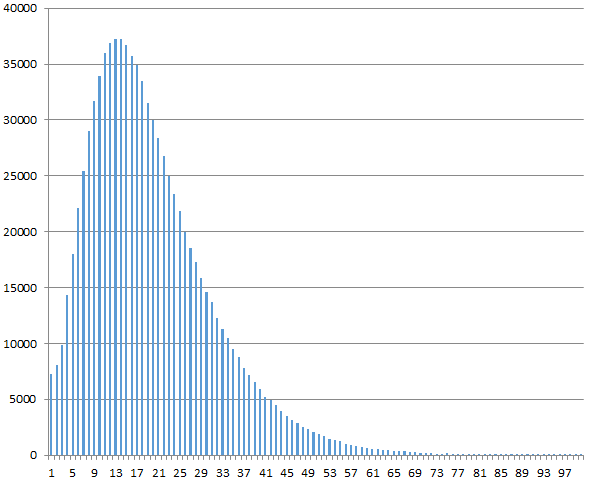
\includegraphics[width=4in]{figures/user_addons_histogram1.png}
\label{fig:distr}
\end{figure}

The data about each addon consisted of:  
\begin{itemize}
    \item {\bf Addon type.} These form a closed set, where prevalent values are `extension', `toolbar', or `BHO' (Browser Helper Object, an Internet Explorer addon). 
    \item {\bf File name.} This includes the full path at which the addon software is installed on the user machine. 
    \item {\bf Name.} Addon's name.
    \item {\bf Description.} A textual description of the addon's functionality.
\end{itemize}

Fig.~\ref{fig:user1} and~\ref{fig:user2} show two addon records associated with two different users. The information specified is browser-dependent and sometimes missing. In these two cases, addon descriptions are missing for the first user and the path information is missing for the second. For each user--addon pair at least one attribute (path, name, or description) is guaranteed to present in the data. 

\begin{figure}[!h]
\caption{{\bf User Addons Record: Sample User 1.}}
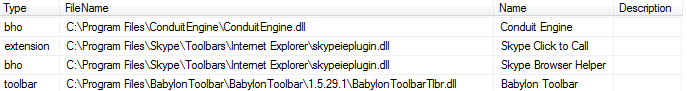
\includegraphics[width=\linewidth]{figures/db_addons_snapshot.png}
\label{fig:user1}
\end{figure}

\begin{figure}[!h]
\caption{{\bf User Addons Record: Sample User 2.}}
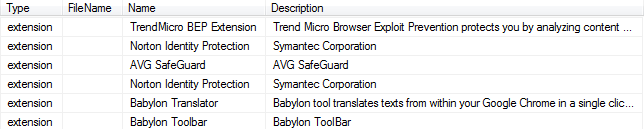
\includegraphics[width=\linewidth]{figures/db_addons_snapshot_desc.png}
\label{fig:user2}
\end{figure}

Importantly, similar addon software may be described by multiple different records, i.e. the addon records lack normalization. Fig.~\ref{fig:example} illustrates this variability across records. Sources of variance include different installation paths, availability or absence of attribute values, and different software version numbers (e.g., 1.8.7.2 vs. 1.6.4.6 in Fig.~\ref{fig:example}). Furthermore, the user base is international and is therefore multilingual. The database includes no tracking of user's or other programs' actions. It was therefore impossible to determine which party initiated the installation (or removal) of an addon.  

\begin{figure}[!h]
\caption{{\bf Example of coreferent addon records with different software version numbers.}}
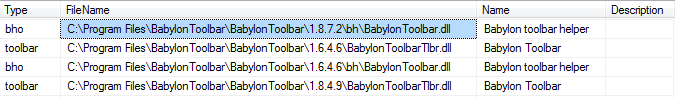
\includegraphics[width=\linewidth]{figures/addons_versioning_snapshot.png}
\label{fig:example}
\end{figure}

\subsection*{Graph representation}

The dataset corresponding to the graph consisted of over 1.3 million nodes and over 18.5 million edges. Detailed statistics are provided in Table~\ref{tab:stat}. The data were represented using a relational graph schema. Each node in the graph represents a unique object that belongs to one of the following node types:   

\begin{enumerate}
\item  \textbf{User. } An individual user is represented as a graph node that carries his/her unique user id. 

\item  \textbf{Addon.  }These nodes correspond to specific addons, defined as the concatenation of all of the addon's attributes; namely, file path, addon name, and description. Addon names often include full file-system path information such as `C:/Program Files (x86)/Skype/skype1.dll'. To avoid registering an addon twice solely due to minor discrepancies in the installation process path prefixes, such as `C://Program Files (x86)/skype', were removed. Additionally, addons with slightly different names, such as different version numbers, were unified for for the random walk. This was done by splitting addon names into tokens and linking the respective \textit{addon} and \textit{term} nodes to maintain connectivity between multiple version of the same \textit{addon}. 

\item  \textbf{Term.  }The text strings that comprise addon names was parsed into individual terms, represented as graph nodes, as illustrated below. 
\end{enumerate}

\begin{table}[!ht]
\centering
\caption{{\bf Graph statistics.}}
\begin{tabular}{|l+l|l|} \hline 
\textbf{Type}  & \textbf{Quantity} \\ \thickhline 
$All\ nodes$  & 1,331,814 \\ \hline 
$User\ nodes$  & 907,844 \\ \hline 
$Addon\ nodes$  & 256,458 \\ \hline 
$Term\ nodes$  & 167,512 \\ \hline 
$High\ degree\ nodes\ (>500)$  & 2,430 \\ \hline 
$All\ edges$  & 18,552,622 \\ \hline 
$User-addon\ edges$  & 17,612,159 \\ \hline 
$Addon-term\ edges$  & 940,463 \\ \hline 
\end{tabular}
\label{tab:stat}
\end{table}

There are two types of edges in the graph. The first type represents the structural association between each \textit{user} and each \textit{addon} installed on his/her machine. The second type links each \textit{addon} node to all \textit{term} nodes that comprise its Bag-of-Terms representation. Inverse edges exist between every connected node pair so the graph may be viewed as undirected. Fig.~\ref{fig:conn} illustrates the graph structure. A \textit{user} is represented as a graph node that is connected to all its corresponding \textit{addon} nodes with undirected edges. Each \textit{addon} node, in turn, is connected to all its \textit{term} nodes. In the specific example of Fig.~\ref{fig:conn}, \textit{user 2} has two addons (\textit{Babylon-addon} and \textit{Conduit-toolbar}) that are connected to their term nodes (\textit{Babylon},\textit{ Conduit},\textit{ addon} and\textit{ toolbar}). To construct the graph, the algorithm iterated over all the users in the dataset to create user nodes. For each user, it then iterated over all his/her addons, and mapped each addon to a unique node. Finally, each \textit{addon} node was tokenized and lower-cased into single words, and each unique word mapped to a respective \textit{term} node.

\begin{figure}[!h]
\caption{{\bf User-Addon-Term connections.}}
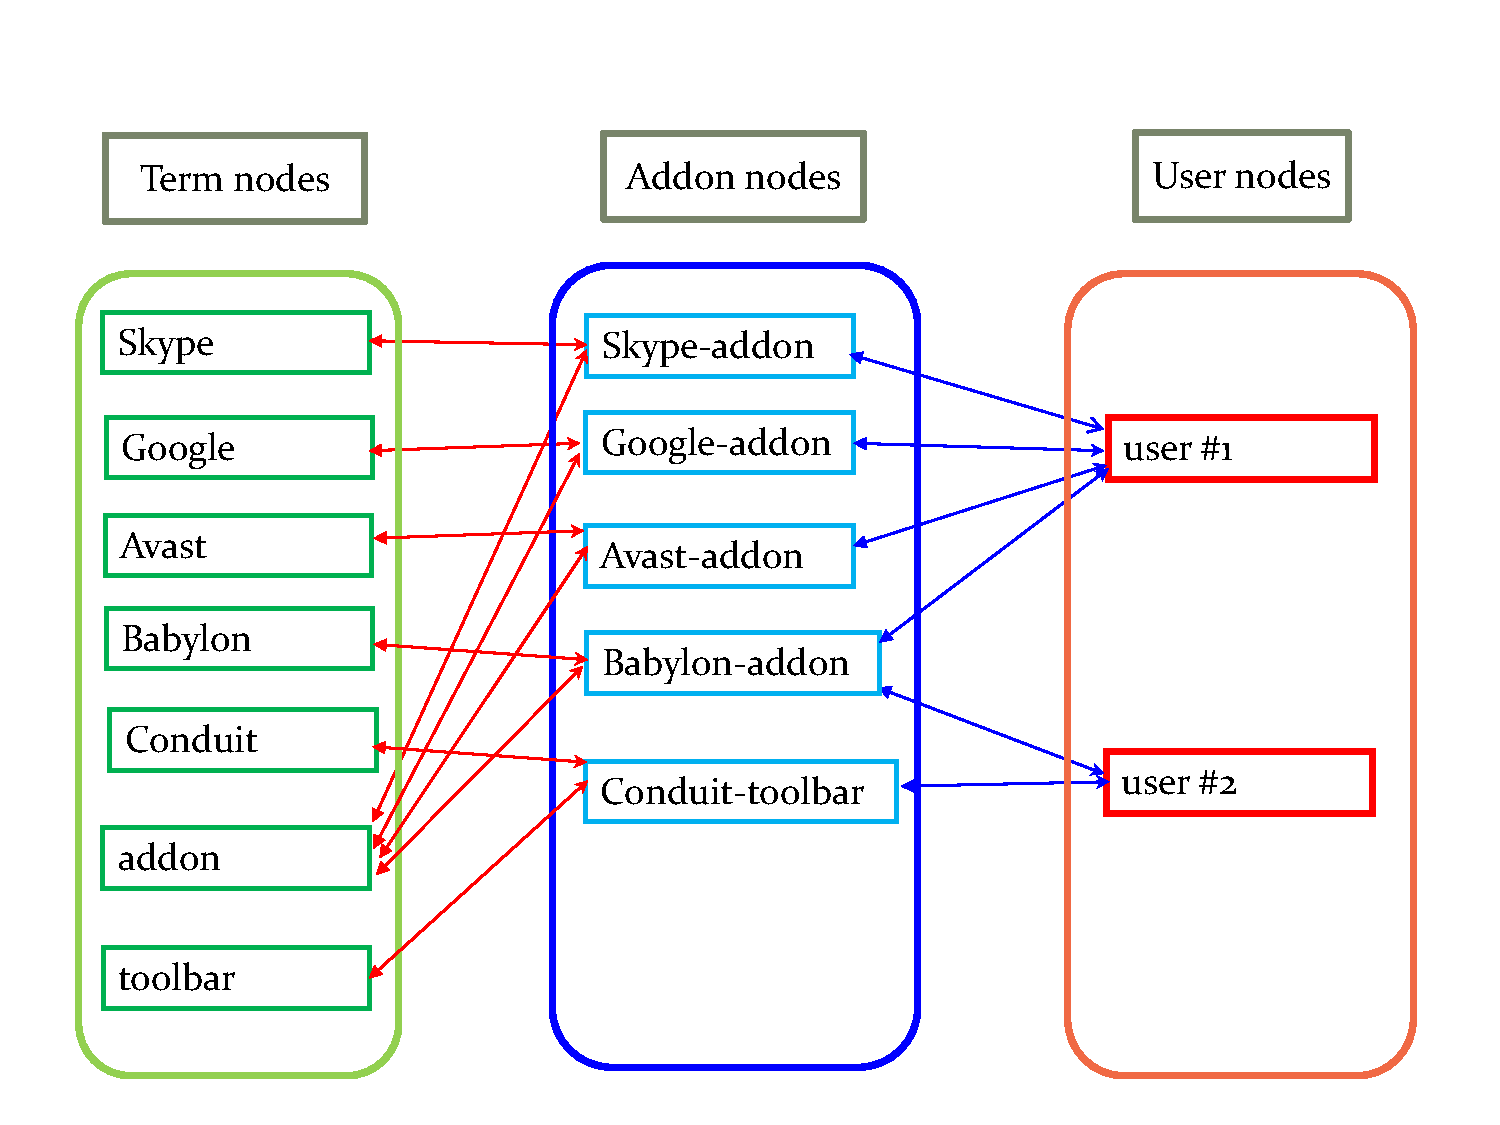
\includegraphics[width=4in]{figures/symbolic_graph.pdf}
\label{fig:conn}
\end{figure}

Besides being compact, the graph representation is advantageous in that similar entities reside in high proximity to each other. Consider, for example, two\textit{ addons} `Skype-US' and `Skype-UK' that have non-identical names, but share the term `Skype' which indicates in this case that they are variants of the same addon. Fig.~\ref{fig:skype} shows how term nodes help construct a connected graph where similar nodes are close to each other. Two disconnected segments on the left panel get connected to each other through the `Skype' term node, which leads to a close relatedness between\textit{ User 1} and\textit{ User 2}. 

\begin{figure}[!h]
\caption{{\bf Example of the constructed graph, without the term layer (left) and with the term layer (right).}}
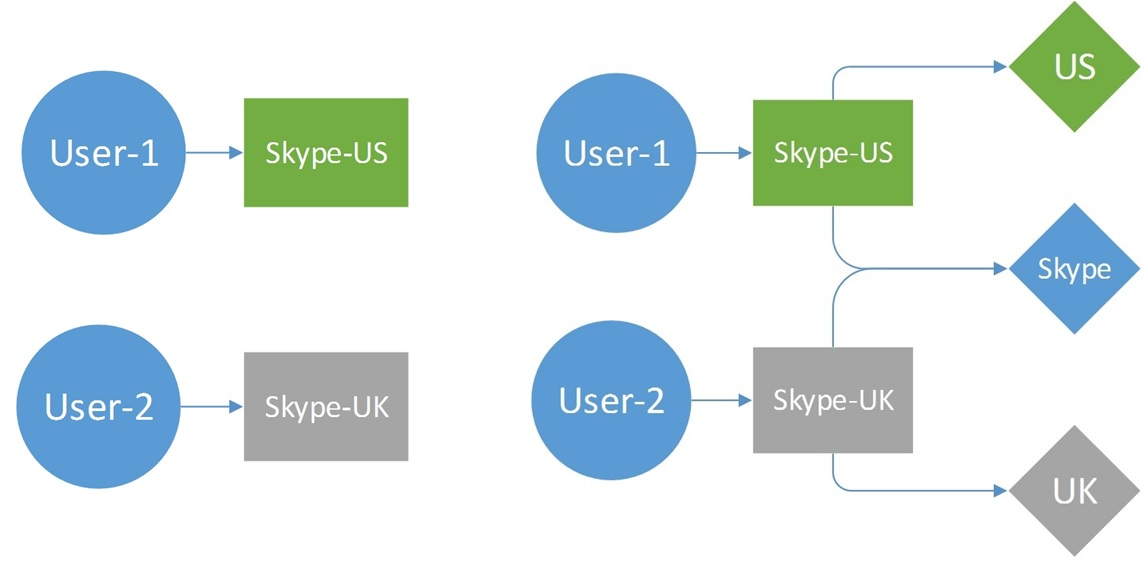
\includegraphics[width=\linewidth]{figures/skype.jpg}
\label{fig:skype}
\end{figure}

\section*{Assessing Research Question 1. Can Web browser habitat resilience be verified?}

Our link prediction experiment for assessing resilience of a browser habitat is designed as follows. A direct link between a \textit{user} and an\textit{ addon} is randomly removed from the graph, and the identity of this `missing' addon is then predicted based on information about remaining \textit{addon} members at the user's environment, applying PPR to rank the \textit{addons} by their graph-based association in the user's environment. The objective of the experiment is to show that PPR can produce significantly better results than an algorithm that does not consider the graph embedded information about users and addons. 

More formally, let $U$ denote the set of users represented as nodes in the underlying graph $G$. Every individual user $u\mathrm{\in }U$ is linked in $G$ to the set of addons installed on $u$'s machine, $A\mathrm{(}u\mathrm{)}$. Having disconnected the link between a random user $u_i$ and an addon $a_j\mathrm{\in }A\mathrm{(}u_i\mathrm{)}$, we wish to evaluate the extent to which the missing link between $u_ia_j$ can be recovered based on the remaining information about the user's environment $A\mathrm{(}u_i\mathrm{)'=}A\mathrm{(}u_i\mathrm{)}\mathrm{\backslash }\mathrm{\{}a_j\}$ and $G$. Using information retrieval terminology, in what follows we will refer to $A\mathrm{(}u_i\mathrm{)'}$ as a \textit{query}. Candidate responses in this case are all\textit{ addons} that are not known to be associated with the user, i.e., $A\backslash A\mathrm{(}u_i\mathrm{)'}$, having this candidate set include the target response $a_j$. These candidate nodes are ranked by their estimated relevance to the query. Accordingly, performance is evaluated quantitatively with respect to the rank of the `missing'\textit{ addon} $a_j$ across multiple instantiated queries.


\subsection*{Approach}

The experiment employs PPR\cite{page1999pagerank} to compute query-specific relevance scores based on the link structure of the graph. An overview of the PPR algorithm can be found in \cite{jeh2003scaling}. In brief, PPR follows the well-known PageRank algorithm that was originally designed to assign a `centrality' score to webpages. PageRank models the behavior of a random surfer who at any given time may choose to either follow a hyperlink to another webpage or to jump (`reset') to some random page on the Web. The probability distribution of finding the surfer at any of the graph nodes at time step $d$ is computed iteratively, as follows: 

\begin{equation} \label{GrindEQ__1_} 
V_{d+1} = (1-\alpha) \left[{1 \over N}\right]_{1 \times N} + \alpha A^\top V_d 
\end{equation} 

\noindent where the total number of nodes (webpages) is $N$, and $A^T$ is a transition matrix that models the probability that the surfer moves to page $j$ from page $i$ following a hyperlink. The probability that the surfer chooses to proceed by following some hyperlink is $\alpha $, and the probability of the alternative action (resetting the walk) is ($\mathrm{1-}\alpha $) . The distribution $V_d$ is guaranteed to converge to a unique stationary distribution $V^{\mathrm{*}}$ in which node scores designate the respective documents' centrality in the network~\cite{page1999pagerank}. In general, a node is assigned a high PageRank score if the sum of the ranks of its backlinks is high, i.e.~if it is linked to by other important webpages.

The PageRank centrality scores reflect the entire network's structure. The\textit{ Personalized PageRank} variant adjusts the random walk model to generate rankings that reflect personal user preferences. Rather than the random surfer reset to any graph node uniformly at random, the reset operation is confined to a subset of graph nodes of interest. Accordingly, the random walk scheme modified as follows: 

\begin{equation} \label{GrindEQ__3_} 
V_{d\mathrm{+1}}\mathrm{=(1-}\alpha \mathrm{)}V_u\mathrm{+}\alpha A^TV_d 
\end{equation} 

\noindent where $V_u$ (the \textit{query}) denotes a distribution over nodes that are of interest to user $u$. PPR scores, derived from the corresponding stationary state distribution, reveal structural similarity, or relevance, of graph nodes with respect to the query nodes. PPR scores for a target node $z$ and any single query node $x$ equal a summation over all the connecting paths between $x$ and $z$ (including cyclic paths, and paths that cross $z$ multiple times) where paths are weighted by their traversal probability~\cite{jeh2003scaling,fogaras2004towards}. In other words, the graph walk distributes probability mass from the start distribution $V_u$ through edges in the graph---incidentally accumulating evidence of similarity over multiple connecting paths. Due to the reset operation, having a fixed fraction of probability mass reassigned to the query nodes at each step, the weights of the paths between $x$ and $z$ exponentially decay as their length increases. This implies that graph nodes that can be reached from the query nodes over shorter connecting paths, as well as over multiple connecting paths, are considered more `important' with respect to the query.


\begin{eqnarray}
\label{eq:schemeP}
	\mathrm{P_Y} = \underbrace{H(Y_n) - H(Y_n|\mathbf{V}^{Y}_{n})}_{S_Y} + \underbrace{H(Y_n|\mathbf{V}^{Y}_{n})- H(Y_n|\mathbf{V}^{X,Y}_{n})}_{T_{X\rightarrow Y}},
\end{eqnarray}

\section*{Materials and Methods}
\subsection*{Etiam eget sapien nibh.}

% For figure citations, please use "Fig" instead of "Figure".
Nulla mi mi, Fig~\ref{fig1} venenatis sed ipsum varius, volutpat euismod diam. Proin rutrum vel massa non gravida. Quisque tempor sem et dignissim rutrum. Lorem ipsum dolor sit amet, consectetur adipiscing elit. Morbi at justo vitae nulla elementum commodo eu id massa. In vitae diam ac augue semper tincidunt eu ut eros. Fusce fringilla erat porttitor lectus cursus, \nameref{S1_Video} vel sagittis arcu lobortis. Aliquam in enim semper, aliquam massa id, cursus neque. Praesent faucibus semper libero.

% Place figure captions after the first paragraph in which they are cited.
\begin{figure}[!h]
\caption{{\bf Bold the figure title.}
Figure caption text here, please use this space for the figure panel descriptions instead of using subfigure commands. A: Lorem ipsum dolor sit amet. B: Consectetur adipiscing elit.}
\label{fig1}
\end{figure}

% Results and Discussion can be combined.
\section*{Results}
Nulla mi mi, venenatis sed ipsum varius, Table~\ref{table1} volutpat euismod diam. Proin rutrum vel massa non gravida. Quisque tempor sem et dignissim rutrum. Lorem ipsum dolor sit amet, consectetur adipiscing elit. Morbi at justo vitae nulla elementum commodo eu id massa. In vitae diam ac augue semper tincidunt eu ut eros. Fusce fringilla erat porttitor lectus cursus, vel sagittis arcu lobortis. Aliquam in enim semper, aliquam massa id, cursus neque. Praesent faucibus semper libero.

% Place tables after the first paragraph in which they are cited.
\begin{table}[!ht]
\begin{adjustwidth}{-2.25in}{0in} % Comment out/remove adjustwidth environment if table fits in text column.
\centering
\caption{
{\bf Table caption Nulla mi mi, venenatis sed ipsum varius, volutpat euismod diam.}}
\begin{tabular}{|l+l|l|l|l|l|l|l|}
\hline
\multicolumn{4}{|l|}{\bf Heading1} & \multicolumn{4}{|l|}{\bf Heading2}\\ \thickhline
$cell1 row1$ & cell2 row 1 & cell3 row 1 & cell4 row 1 & cell5 row 1 & cell6 row 1 & cell7 row 1 & cell8 row 1\\ \hline
$cell1 row2$ & cell2 row 2 & cell3 row 2 & cell4 row 2 & cell5 row 2 & cell6 row 2 & cell7 row 2 & cell8 row 2\\ \hline
$cell1 row3$ & cell2 row 3 & cell3 row 3 & cell4 row 3 & cell5 row 3 & cell6 row 3 & cell7 row 3 & cell8 row 3\\ \hline
\end{tabular}
\begin{flushleft} Table notes Phasellus venenatis, tortor nec vestibulum mattis, massa tortor interdum felis, nec pellentesque metus tortor nec nisl. Ut ornare mauris tellus, vel dapibus arcu suscipit sed.
\end{flushleft}
\label{table1}
\end{adjustwidth}
\end{table}


%PLOS does not support heading levels beyond the 3rd (no 4th level headings).
\subsection*{\lorem\ and \ipsum\ Nunc blandit a tortor.}
\subsubsection*{3rd Level Heading.} 
Maecenas convallis mauris sit amet sem ultrices gravida. Etiam eget sapien nibh. Sed ac ipsum eget enim egestas ullamcorper nec euismod ligula. Curabitur fringilla pulvinar lectus consectetur pellentesque. Quisque augue sem, tincidunt sit amet feugiat eget, ullamcorper sed velit. Sed non aliquet felis. Lorem ipsum dolor sit amet, consectetur adipiscing elit. Mauris commodo justo ac dui pretium imperdiet. Sed suscipit iaculis mi at feugiat. 

\begin{enumerate}
	\item{react}
	\item{diffuse free particles}
	\item{increment time by dt and go to 1}
\end{enumerate}


\subsection*{Sed ac quam id nisi malesuada congue.}

Nulla mi mi, venenatis sed ipsum varius, volutpat euismod diam. Proin rutrum vel massa non gravida. Quisque tempor sem et dignissim rutrum. Lorem ipsum dolor sit amet, consectetur adipiscing elit. Morbi at justo vitae nulla elementum commodo eu id massa. In vitae diam ac augue semper tincidunt eu ut eros. Fusce fringilla erat porttitor lectus cursus, vel sagittis arcu lobortis. Aliquam in enim semper, aliquam massa id, cursus neque. Praesent faucibus semper libero.

\begin{itemize}
	\item First bulleted item.
	\item Second bulleted item.
	\item Third bulleted item.
\end{itemize}

\section*{Discussion}
Nulla mi mi, venenatis sed ipsum varius, Table~\ref{table1} volutpat euismod diam. Proin rutrum vel massa non gravida. Quisque tempor sem et dignissim rutrum. Lorem ipsum dolor sit amet, consectetur adipiscing elit. Morbi at justo vitae nulla elementum commodo eu id massa. In vitae diam ac augue semper tincidunt eu ut eros. Fusce fringilla erat porttitor lectus cursus, vel sagittis arcu lobortis. Aliquam in enim semper, aliquam massa id, cursus neque. Praesent faucibus semper libero~\cite{bib3}.

\section*{Conclusion}

CO\textsubscript{2} Maecenas convallis mauris sit amet sem ultrices gravida. Etiam eget sapien nibh. Sed ac ipsum eget enim egestas ullamcorper nec euismod ligula. Curabitur fringilla pulvinar lectus consectetur pellentesque. Quisque augue sem, tincidunt sit amet feugiat eget, ullamcorper sed velit. 

Sed non aliquet felis. Lorem ipsum dolor sit amet, consectetur adipiscing elit. Mauris commodo justo ac dui pretium imperdiet. Sed suscipit iaculis mi at feugiat. Ut neque ipsum, luctus id lacus ut, laoreet scelerisque urna. Phasellus venenatis, tortor nec vestibulum mattis, massa tortor interdum felis, nec pellentesque metus tortor nec nisl. Ut ornare mauris tellus, vel dapibus arcu suscipit sed. Nam condimentum sem eget mollis euismod. Nullam dui urna, gravida venenatis dui et, tincidunt sodales ex. Nunc est dui, sodales sed mauris nec, auctor sagittis leo. Aliquam tincidunt, ex in facilisis elementum, libero lectus luctus est, non vulputate nisl augue at dolor. For more information, see \nameref{S1_Appendix}.

\section*{Supporting Information}

% Include only the SI item label in the paragraph heading. Use the \nameref{label} command to cite SI items in the text.
\paragraph*{S1 Fig.}
\label{S1_Fig}
{\bf Bold the title sentence.} Add descriptive text after the title of the item (optional).

\paragraph*{S2 Fig.}
\label{S2_Fig}
{\bf Lorem Ipsum.} Maecenas convallis mauris sit amet sem ultrices gravida. Etiam eget sapien nibh. Sed ac ipsum eget enim egestas ullamcorper nec euismod ligula. Curabitur fringilla pulvinar lectus consectetur pellentesque.

\paragraph*{S1 File.}
\label{S1_File}
{\bf Lorem Ipsum.}  Maecenas convallis mauris sit amet sem ultrices gravida. Etiam eget sapien nibh. Sed ac ipsum eget enim egestas ullamcorper nec euismod ligula. Curabitur fringilla pulvinar lectus consectetur pellentesque.

\paragraph*{S1 Video.}
\label{S1_Video}
{\bf Lorem Ipsum.}  Maecenas convallis mauris sit amet sem ultrices gravida. Etiam eget sapien nibh. Sed ac ipsum eget enim egestas ullamcorper nec euismod ligula. Curabitur fringilla pulvinar lectus consectetur pellentesque.

\paragraph*{S1 Appendix.}
\label{S1_Appendix}
{\bf Lorem Ipsum.} Maecenas convallis mauris sit amet sem ultrices gravida. Etiam eget sapien nibh. Sed ac ipsum eget enim egestas ullamcorper nec euismod ligula. Curabitur fringilla pulvinar lectus consectetur pellentesque.

\paragraph*{S1 Table.}
\label{S1_Table}
{\bf Lorem Ipsum.} Maecenas convallis mauris sit amet sem ultrices gravida. Etiam eget sapien nibh. Sed ac ipsum eget enim egestas ullamcorper nec euismod ligula. Curabitur fringilla pulvinar lectus consectetur pellentesque.

\section*{Acknowledgments}
Cras egestas velit mauris, eu mollis turpis pellentesque sit amet. Interdum et malesuada fames ac ante ipsum primis in faucibus. Nam id pretium nisi. Sed ac quam id nisi malesuada congue. Sed interdum aliquet augue, at pellentesque quam rhoncus vitae.

\nolinenumbers

% Either type in your references using
% \begin{thebibliography}{}
% \bibitem{}
% Text
% \end{thebibliography}
%
% or
%
% Compile your BiBTeX database using our plos2015.bst
% style file and paste the contents of your .bbl file
% here.
% 
\bibliographystyle{plos2015}
\bibliography{plos}


\end{document}

